\documentclass[a4paper,12pt]{article}
%%%%%%%%%%%%%%%%%%%%%%%%%%%%%%%%%%%%%%%%%%%%%%%%%%%%%%%%%%%%%%%%%%%%%%%%%%%%%%%%%%%%%%%%%%%%%%%%%%%%%%%%%%%%%%%%%%%%%%%%%%%%%%%%%%%%%%%%%%%%%%%%%%%%%%%%%%%%%%%%%%%%%%%%%%%%%%%%%%%%%%%%%%%%%%%%%%%%%%%%%%%%%%%%%%%%%%%%%%%%%%%%%%%%%%%%%%%%%%%%%%%%%%%%%%%%
\usepackage{eurosym}
\usepackage{vmargin}
\usepackage{amsmath}
\usepackage{graphics}
\usepackage{epsfig}
\usepackage{framed}
\usepackage{subfigure}
\usepackage{fancyhdr}

\setcounter{MaxMatrixCols}{10}
%TCIDATA{OutputFilter=LATEX.DLL}
%TCIDATA{Version=5.00.0.2570}
%TCIDATA{<META NAME="SaveForMode"CONTENT="1">}
%TCIDATA{LastRevised=Wednesday, February 23, 201113:24:34}
%TCIDATA{<META NAME="GraphicsSave" CONTENT="32">}
%TCIDATA{Language=American English}

\pagestyle{fancy}
\setmarginsrb{20mm}{0mm}{20mm}{25mm}{12mm}{11mm}{0mm}{11mm}
\lhead{Advanced Data Modelling} \rhead{Logistic Regression} \chead{MA4128} %\input{tcilatex}

%http://www.electronics.dit.ie/staff/ysemenova/Opto2/CO_IntroLab.pdf
\begin{document}
	\Large


\section{Binary Logistic Regression}
Binary Logistic regression is used to determine the impact of multiple independent variables
presented simultaneously to predict membership of one or other of the two
dependent variable categories.

\subsection{Likelihood Ratio Test}
The likelihood ratio test is a test of the difference between –2LL for the full
model with predictors and –2LL for initial chi-square in the null model.
When probability fails to reach the 5\% significance level, we retain the null hypothesis
that knowing the independent variables (predictors) has no increased effects (i.e. make no
difference) in predicting the dependent.

\subsection{Psuedo R Squared Values}
%http://statistics.ats.ucla.edu/stat/mult_pkg/faq/general/Psuedo_RSquareds.htm


\subsection{The Hosmer-Lemeshow Test}
%http://www.strath.ac.uk/aer/materials/5furtherquantitativeresearchdesignandanalysis/unit6/goodnessoffitmeasures/

The Hosmer-Lemeshow test of goodness of fit is not automatically a part of the SPSS logistic regression output. To get this output, we need to go into `\textbf{\texttt{options}}’ and tick the box marked Hosmer-Lemeshow test of goodness of fit. In our example, this gives us the following output:

\begin{tabular}{|c|c|c|c|}
\hline  Step	& Chi-square&	df 	 & Sig. \\ \hline
 1	 & 142.032	& 6	 &.000 \\ 
\hline 
\end{tabular} 

Therefore, our model is significant, suggesting it does not fit the data. However, as we have a sample size of over 13,000, even very small divergencies of the model from the data would be flagged up and cause significance. Therefore, with samples of this size it is hard to find models that are parsimonious (i.e. that use the minimum amount of independent variables to explain the dependent variable) and fit the data. Therefore, other fit indices might be more appropriate.

% Binary Regression : http://teaching.sociology.ul.ie/SSS/lugano/node10.html 
% http://istics.net/pdfs/multivariate.pdf
%---------------------------------------------------------- %
\section{Logistic Regression}
Logistic regression, also called a logit model, is used to model \textbf{dichotomous outcome} variables. 
In the logit model the \textbf{log odds} of the outcome is modeled as a linear combination of the predictor variables.

In logistic regression theory, the predicted dependent variable is a function of the probability that a particular subject will be in one of the categories (for example, the probability that a patient has the disease, given his or her set of scores on the predictor variables).

%---------------------------------------------------------- %
\subsection{Introduction to the Odds Ratio}
Let's begin with probability.  Let's say that the probability of success is 0.8, thus
p = 0.8
Then the probability of failure is
\[q = 1 - p = 0.2\]
The odds of success are defined as
\[odds(success) = p/q = 0.8/0.2 = 4\]
that is, the odds of success are 4 to 1. The odds of failure would be
\[odds(failure) = q/p = .2/.8 = .25\]
This looks a little strange but it is really saying that the odds of failure are 1 to 4.  The odds of success and the odds of failure are just reciprocals of one another, i.e., 1/4 = .25 and 1/.25 = 4. 


 Next, we will add another variable to the equation so that we can compute an odds ratio.

\textbf{Another example}

Suppose that seven out of 10 males are admitted to an engineering school while three of 10 females are admitted. 

\begin{itemize}
\item The probabilities for admitting a male are,
p = 7/10 = .7      ( q = 1 - .7 = .3)
\item Here are the same probabilities for females,
p = 3/10 = .3       (q = 1 - .3 = .7)
\end{itemize}
Now we can use the probabilities to compute the admission odds for both males and females,
\begin{itemize}
\item odds(male) = .7/.3 = 2.33333
\item odds(female) = .3/.7 = .42857
\end{itemize}
Next, we compute the odds ratio for admission,
\[OR = 2.3333/0.42857 = 5.44\]
Thus, for a male, the odds of being admitted are 5.44 times as large than the odds for a female being admitted.

\subsection{About logits}


There is a direct relationship between the coefficients produced by \textbf{logit} and the odds ratios produced by the logistic procedure.  First, let's define what is meant by a logit:  A logit is defined as the log base e (log) of the odds,
\[logit(p) = log(odds) = log(p/q)\]
Logistic regression is in reality ordinary regression using the logit as the response variable,

\[logit(p) = a + bX\]
\[log(p/q) = a + bX\]
This means that the coefficients in logistic regression are in terms of the log odds, that is, the coefficient 1.694596 implies that a one unit change in gender results in a 1.694596 unit change in the log of the odds.  

Equation [3] can be expressed in odds by getting rid of the log.  This is done by taking e to the power for both sides of the equation.
\[ p/q = e^{a + bX}\]
The end result of all the mathematical manipulations is that the odds ratio can be computed by raising e to the power of the logistic coefficient,
   \[OR = e^b = e^1.694596 = 5.44\]
%------------------------------------------------------------------------------------------------------------------------- %
\subsection{Logistic Regression: Odds Ratio}
What are odds?
The odds of outcome 1 versus outcome 2 are the probability (or frequency) of outcome 1 divided by the probability (or frequency) of outcome 2.


\[ \hat{Y} = \frac{\mbox{Odds}}{1+\mbox{Odds}} \]


Loglinear models essentially define a pattern of odds ratios, apply the marginals to them, and compare the resulting table with the observed table, in pretty much the same way we apply the Pearson  $\chi^2$ test for association. The big difference is the pattern we define can be much more complicated than independence.

%---------------------------------------------------------- %
\newpage
\section{The Wald Test}

The Wald test is a way of testing the significance of particular explanatory variables in a statistical model. 

In logistic regression we have a binary outcome variable and one or more explanatory variables. For each explanatory variable in the model there will be an associated parameter. The Wald test is one of a number of ways of testing whether the parameters associated with a group of explanatory variables are zero.
%, described by Polit (1996) and Agresti (1990), 

If for a particular explanatory variable, or group of explanatory variables, the Wald test is significant, then we would conclude that the parameters associated with these variables are not zero, so that the variables should be included in the model. If the Wald test is not significant then these explanatory variables can be omitted from the model. 

When considering a single explanatory variable, Altman (1991) uses a t-test to check whether the parameter is significant. For a single parameter the Wald statistic is just the square of the t-statistic and so will give exactly equivalent results.

An alternative and widely used approach to testing the signi®cance of a number of explanatory variables is to use the likelihood ratio test. This is appropriate for a variety of types of statistical models. 

Agresti (1990) argues that the likelihood ratio test is better, particularly if the sample size is small or the parameters are large.

\subsection{Logistic Regression}

%[\ \pi(x) = \frac{e^{(\beta_0 + \beta_1 x)}} {e^{(\beta_0 + \beta_1 x)} + 1} = \frac {1} {e^{-(\beta_0 + \beta_1 x)} + 1},\]
and

\[g(x) = \ln \frac {\pi(x)} {1 - \pi(x)} = \beta_0 + \beta_1 x ,\]

and

\[\frac{\pi(x)} {1 - \pi(x)} = e^{(\beta_0 + \beta_1 x)}.\]

\subsection{Wald statistic}

Alternatively, when assessing the contribution of individual predictors in a given model, one may examine the significance of the Wald statistic. The Wald statistic, analogous to the t-test in linear regression, is used to assess the significance of coefficients. The Wald statistic is the ratio of the square of the regression coefficient to the square of the standard error of the coefficient and is asymptotically distributed as a chi-square distribution.

\subsection{Pseudo-R Squared}
Cox  and Snell R Square and Nagelkerke R Square - These are pseudo R-squares.  Logistic regression does not have an equivalent to the R-squared that is found in OLS regression; however, many people have tried to come up with one.  

There are a wide variety of pseudo-R-square statistics (these are only two of them).  Because this statistic does not mean what R-squared means in OLS regression (the proportion of variance explained by the predictors), we suggest interpreting this statistic with great caution.
%---------------------------------------------------------- %
\newpage
\subsection{Logistic Regression: Decision Rule}
Our decision rule will take the following form: If the probability of the event is greater than or equal to some threshold, we shall predict that the event will take place. By default, SPSS sets this threshold to .5. While that seems reasonable, in many cases we may want to set it higher or lower than .5.

%---------------------------------------------------------- %
\section{Multinomial Logistic Regression}
Examples of multinomial logistic regression

Example 1. People's occupational choices might be influenced by their parents' occupations and their own education level. We can study the relationship of one's occupation choice with education level and father's occupation.  The occupational choices will be the outcome variable which consists of categories of occupations.

Example 2. A biologist may be interested in food choices that alligators make. Adult alligators might have difference preference than young ones. The outcome variable here will be the types of food, and the predictor variables might be the length of the alligators and other environmental variables.

Example 3. Entering high school students make program choices among general program, vocational program and academic program. Their choice might be modeled using their writing score and their social economic status.
%---------------------------------------------------------- %

\subsection{Classification Plot} 
The classification plot or histogram of predicted probabilities
provides a visual demonstration of the correct and incorrect predictions. Also called the ‘classplot’ or the ‘plot of observed groups and predicted probabilities’,it is another very useful piece of information from the SPSS output when one chooses
‘Classification plots’ under the Options button in the Logistic Regression dialogue box.

\newpage

\begin{framed}
	
	\subsubsection*{Types of Variables (Revision)}
	\begin{itemize}
		\item Examples of \textbf{continuous variables} include revision time (measured in hours), intelligence (measured using IQ score), exam performance (measured from 0 to 100), weight (measured in kg), and so forth. 
		
		\item Examples of \textbf{ordinal variables} include \textit{Likert} items (e.g., a 7-point scale from "strongly agree" through to "strongly disagree"), amongst other ways of ranking categories (e.g., a 3-point scale explaining how much a customer liked a product, ranging from "Not very much" to "Yes, a lot"). 
		\item Examples of \textbf{nominal variables} include gender (e.g., 2 groups: male and female), ethnicity (e.g., 3 groups: Caucasian, African American and Hispanic), profession (e.g., 5 groups: surgeon, doctor, nurse, dentist, therapist), and so forth.
	\end{itemize}
\end{framed}
\newpage
\section*{Introduction to Logistic Regression}

Logistic regression determines the impact of multiple independent variables
presented simultaneously to predict membership of one or other of the two
dependent variable categories.

\section{Binomial Logistic Regression} 
A binomial logistic regression (often referred to simply as logistic regression), predicts the probability that an observation falls into one of two categories of a \textbf{dichotomous} dependent variable based on one or more independent variables that can be either continuous or categorical.

\section{Binomial Logistic Regression: Model Diagnostics}

\begin{itemize}
	\item In order to understand how much variation in the dependent variable can be explained by the model (the equivalent of $R^2$ in multiple regression), you sho$R^2$uld consult Model Summary statistics.
	
	\item The SPSS output table below contains the \textit{Cox \& Snell R Square} and \textit{Nagelkerke R Square }values, which are both methods of calculating the explained variation. These values are sometimes referred to as pseudo $R^2$ values (and will have lower values than in multiple regression).
	\item  However, they are interpreted in the same manner, but with more caution. Therefore, the explained variation in the dependent variable based on our model ranges from 24.0\% to 33.0\%, depending on whether you reference the Cox \& Snell $R^2$ or Nagelkerke $R^2$ methods, respectively. 
	
	\item Nagelkerke $R^2$ is a modification of Cox \& Snell $R^2$, the latter of which cannot achieve a value of 1. For this reason, it is preferable to report the Nagelkerke $R^2$ value.
\end{itemize}

\begin{figure}[h!]
\centering
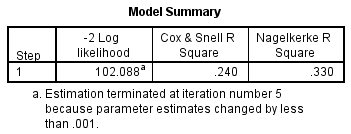
\includegraphics[width=0.9\linewidth]{images/BLogReg-Rsq}
\caption{SPSS output}
\label{fig:BLogReg-Rsq}
\end{figure}



\section*{Logistic function} 

The logistic function, with $\beta_0 + \beta_1 x$ on the horizontal axis and $\pi(x)$ on the vertical axis
An explanation of logistic regression begins with an explanation of the logistic function, which always takes on values between zero and one:
\[
F(t) = \frac{e^t}{e^t+1} = \frac{1}{1+e^{-t}},
\]
and viewing t as a linear function of an explanatory variable x (or of a linear combination of explanatory variables), the logistic function can be written as:
\[\pi(x) = \frac{e^{(\beta_0 + \beta_1 x)}} {e^{(\beta_0 + \beta_1 x)} + 1} = \frac {1} {1+e^{-(\beta_0 + \beta_1 x)}}.
\]
This will be interpreted as the probability of the dependent variable equalling a "success" or "case" rather than a failure or non-case. We also define the inverse of the logistic function, the logit:
\[g(x) = \ln \frac {\pi(x)} {1 - \pi(x)} = \beta_0 + \beta_1 x ,
\]and equivalently:
\[\frac{\pi(x)} {1 - \pi(x)} = e^{(\beta_0 + \beta_1 x)}.
\]



\section{Binomial Logistic Regression}
Binomial logistic regression estimates the probability of an event (as an example, having heart disease) occurring. 
\begin{itemize}
	\item If the estimated probability of the event occurring is greater than or equal to 0.5 (better than even chance), the procedure classifies the event as occurring (e.g., heart disease being present). \item If the probability is less than 0.5, Logistic regression classifies the event as not occurring (e.g., no heart disease). 
\end{itemize}
\subsection{Category Prediction Table}




It is very common to use binomial logistic regression to predict whether cases can be correctly classified (i.e., predicted) from the independent variables. Therefore, it becomes necessary to have a method to assess the effectiveness of the predicted classification against the actual classification. There are many methods to assess this with their usefulness oftening depending on the nature of the study conducted. However, all methods revolve around the observed and predicted classifications, which are presented in the ``Classification Table", as shown below:


\begin{figure}
\centering
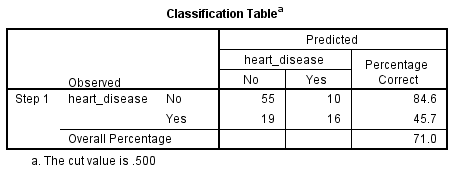
\includegraphics[width=0.7\linewidth]{images/BLogReg-Table}
\caption{}
\label{fig:BLogReg-Table}
\end{figure}



Firstly, notice that the table has a subscript which states, ``The cut value is .500". This means that if the probability of a case being classified into the "yes" category is greater than .500, then that particular case is classified into the "yes" category. 
Otherwise, the case is classified as in the "no" category. 

\subsection{Interpreting the Classifcation Table}
Whilst the classification table appears to be very simple, it actually provides a lot of important information about your binomial logistic regression result, including:


\begin{itemize}
	\item[A.] The \textbf{percentage accuracy in classification (PAC)}, which reflects the percentage of cases that can be correctly classified as "no" heart disease with the independent variables added (not just the overall model).
	\item[B.] \textbf{Sensitivity}, which is the percentage of cases that had the observed characteristic (e.g., "yes" for heart disease) which were correctly predicted by the model (i.e., true positives).
	\item[C.] \textbf{Specificity}, which is the percentage of cases that did not have the observed characteristic (e.g., "no" for heart disease) and were also correctly predicted as not having the observed characteristic (i.e., true negatives).
	\item[D.] The \textbf{positive predictive value}, which is the percentage of correctly predicted cases "with" the observed characteristic compared to the total number of cases predicted as having the characteristic.
	\item[E.] The \textbf{negative predictive value}, which is the percentage of correctly predicted cases ``without" the observed characteristic compared to the total number of cases predicted as not having the characteristic.
\end{itemize}
%--------------------------------------------------------------------------------------%


\section{Introduction to Logistic Regression}
\begin{itemize}
	\item Logistic regression or logit regression is a type of probabilistic statistical classification model.
	
	\item It is also used to predict a binary response from a binary predictor, used for predicting the outcome of a categorical dependent variable (i.e., a class label) based on one or more predictor variables (features). 
	
	\item That is, it is used in estimating empirical values of the parameters in a qualitative response model. The probabilities describing the possible outcomes of a single trial are modeled, as a function of the explanatory (predictor) variables, using a logistic function. 
	
	\item Logistic regression, also called a logit model, is used to model \textbf{dichotomous (i.e. Binary) outcome variables}. In the logit model the log odds of the outcome is modeled as a linear combination of the predictor variables.
\end{itemize}


\subsection{Examples of Logistic Regression}

\begin{description}
	\item[Example 1:]  Suppose that we are interested in the factors that influence whether a political candidate wins an election.  The outcome (response) variable is binary (0/1); \textit{ win or lose}.  The predictor variables of interest are the amount of money spent on the campaign, the amount of time spent campaigning negatively and whether or not the candidate is an incumbent.
	
	\item[Example 2:]  A researcher is interested in how variables, such as GRE (Graduate Record Exam scores), GPA (grade point average) and prestige of the undergraduate institution, effect admission into graduate school. The response variable, \textit{admit/don't admit}, is a binary variable.
\end{description}

%You could use binomial logistic regression to understand whether exam performance can be predicted based on revision time, test anxiety and lecture attendance (i.e., where the dependent variable is ``exam performance", measured on a dichotomous scale – ``passed" or ``failed" – and you have three independent variables: ``revision time", ``test anxiety" and ``lecture attendance"). 
%
%
%Alternately, you could use binomial logistic regression to understand whether drug use can be predicted based on prior criminal convictions, drug use amongst friends, income, age and gender (i.e., where the dependent variable is ``drug use", measured on a dichotomous scale – ``yes" or ``no" – and you have five independent variables: ``prior criminal convictions", ``drug use amongst friends", ``income", ``age" and "gender").
\newpage
\subsection{Assumptions}

\begin{description}
	\item[Assumption 1:] Your dependent variable should be measured on a \textbf{dichotomous scale}. Examples of dichotomous variables include gender (two groups: "males" and "females"), presence of heart disease (two groups: "yes" and "no"), personality type (two groups: "introversion" or "extroversion"), body composition (two groups: "obese" or "not obese"), and so forth. \\
	\newline
	However, if your dependent variable was not measured on a dichotomous scale, but a continuous scale instead, you will need to carry out \textbf{multiple regression}, whereas if your dependent variable was measured on an ordinal scale, \textbf{ordinal regression} would be a more appropriate starting point.
	
	\item[Assumption 2:] You have one or more independent variables, which can be either continuous (i.e., an interval or ratio variable) or categorical (i.e., an ordinal or nominal variable). 
	
	
	
	\item[Assumption 3:] You should have independence of observations and the dependent variable should have mutually exclusive and exhaustive categories.
	
	\item[Assumption 4:] There needs to be a linear relationship between any continuous independent variables and the logit transformation of the dependent variable. 
\end{description}

%----------------------------------------------------------------------------------------%


\section{Logistic Regression: Odds Ratios and Log-Odds}
\begin{itemize}
	\item Suppose that in a sample of 100 men, 90 drank wine in the previous week, while in a sample of 100 women only 20 drank wine in the same period. \item The odds of a man drinking wine are 90 to 10, or 9:1, while the odds of a woman drinking wine are only 20 to 80, or 1:4 = 0.25:1. 
	\item The odds ratio is thus 9/0.25, or 36, showing that men are much more likely to drink wine than women. 
	\item The detailed calculation is:
	
	
	\[ { 0.9/0.1 \over 0.2/0.8}=\frac{\;0.9\times 0.8\;}{\;0.1\times 0.2\;} ={0.72 \over 0.02} = 36 \]
	
	\item This example also shows how odds ratios are sometimes sensitive in stating relative positions: in this sample men are 90/20 = 4.5 times more likely to have drunk wine than women, but have 36 times the odds. 
	
	
	
	\item The logarithm of the odds ratio, the difference of the logits of the probabilities, tempers this effect, and also makes the measure symmetric with respect to the ordering of groups. 
	\item For example, using natural logarithms, an odds ratio of 36/1 maps to 3.584, and an odds ratio of 1/36 maps to -3.584.
\end{itemize}


\section*{Logistic Regression: Logit Transformation}
%http://data.princeton.edu/wws509/notes/c3.pdf

The logit transformation is given by the following formula: 
\[ \eta_i = \mbox{logit}(\pi_i)  = \mbox{log}\left( \frac{\pi_i}{1- \pi_i} \right) \]

\noindent 
The inverse of the logit transformation is given by the following formula: 
\[ \pi_i = \mbox{logit}^{-1}(\eta_i)  =  \frac{e^{\eta_i}}{1 + e^{\eta_i}} \]

%---------------------------%
\subsection*{Example 1}
Given that $\pi_i = 0.2$, compute $\eta_i$.

\[ \eta_i = \mbox{log}\left( \frac{0.2}{1-0.2} \right)= \mbox{log}\left( \frac{0.2}{0.8} \right)\] 

\[ \eta_i =  \mbox{log}(0.25) =-1.386 \]

%---------------------------%
\subsection*{Example 2}
Given that $\eta_i = 2.3$, compute $\pi_i$.

\[ \pi_i  =  \frac{e^{2.3}}{1 + e^{2.3}} = \frac{9.974}{1 + 9.974} = 0.908 \]

%--------------------------------------------------------------------------------------%

\subsection*{Logits}
In logistic regression, the logit may be computed in a manner similar to linear regression:
\[ \eta_i = \beta_0 + \beta_1x_1 + \beta_2x_2 + \ldots  \]

%---------------------------%

\section{Logistic Regression: Odds Ratios and Log-Odds}
\begin{itemize}
	\item Suppose that in a sample of 100 men, 90 drank wine in the previous week, while in a sample of 100 women only 20 drank wine in the same period. The odds of a man drinking wine are 90 to 10, or 9:1, while the odds of a woman drinking wine are only 20 to 80, or 1:4 = 0.25:1. 
	\item The odds ratio is thus 9/0.25, or 36, showing that men are much more likely to drink wine than women. The detailed calculation is:
	
	\[ { 0.9/0.1 \over 0.2/0.8}=\frac{\;0.9\times 0.8\;}{\;0.1\times 0.2\;} ={0.72 \over 0.02} = 36 \]
	
	\item This example also shows how odds ratios are sometimes sensitive in stating relative positions: in this sample men are 90/20 = 4.5 times more likely to have drunk wine than women, but have 36 times the odds. 
	
	
	\item The logarithm of the odds ratio, the difference of the logits of the probabilities, tempers this effect, and also makes the measure symmetric with respect to the ordering of groups. For example, using natural logarithms, an odds ratio of 36/1 maps to 3.584, and an odds ratio of 1/36 maps to -3.584.
\end{itemize}



\section*{Logistic function} 

The logistic function, with $\beta_0 + \beta_1 x$ on the horizontal axis and $\pi(x)$ on the vertical axis
An explanation of logistic regression begins with an explanation of the logistic function, which always takes on values between zero and one:
\[
F(t) = \frac{e^t}{e^t+1} = \frac{1}{1+e^{-t}},
\]
and viewing t as a linear function of an explanatory variable x (or of a linear combination of explanatory variables), the logistic function can be written as:
\[\pi(x) = \frac{e^{(\beta_0 + \beta_1 x)}} {e^{(\beta_0 + \beta_1 x)} + 1} = \frac {1} {1+e^{-(\beta_0 + \beta_1 x)}}.
\]
This will be interpreted as the probability of the dependent variable equalling a ``success" or ``case" rather than a failure or non-case. We also define the inverse of the logistic function, the logit:
\[g(x) = \ln \frac {\pi(x)} {1 - \pi(x)} = \beta_0 + \beta_1 x ,
\]and equivalently:
\[\frac{\pi(x)} {1 - \pi(x)} = e^{(\beta_0 + \beta_1 x)}.
\]
%======================================================%

\section{Logistic Regression: Logits}
%http://data.princeton.edu/wws509/notes/c3.pdf

The logit transformation is given by the following formula: 
\[ \eta_i = \mbox{logit}(\pi_i)  = \mbox{log}\left( \frac{\pi_i}{1- \pi_i} \right) \]

To inverse of the logit transformation is given by the following formula: 
\[ \pi_i = \mbox{logit}^{-1}(\eta_i)  =  \frac{e^{\eta_i}}{1 + e^{\eta_i}} \]

%---------------------------%

\subsection{Example 2}
Let us suppose that the probability of survival of a marine species of fauna is dependent on pollution, depth and water temperature. Suppose the logit for the logistic regression was computed as follows:
\[ \eta_i = 0.14 + 0.76x_1 - 0.093x_2 + 1.2x_3  \]
\begin{center}
	\begin{tabular}{|c|c|c|}
		\hline
		% after \\: \hline or \cline{col1-col2} \cline{col3-col4} ...
		Variables & case 1 & case 2 \\ \hline
		Pollution($x_1$) & 6.0 & 1.9 \\
		Depth ($x_2$)& 51 & 99 \\
		Temp ($x_3$) & 3.0 & 2.9 \\
		\hline
	\end{tabular}
\end{center}
Compute the probability of success for both case 1 and case 2.

\begin{itemize}
	\item case 1$ \eta_1 = 0.14 + (0.76 \times 6)	- (0.093\times 51) + (1.2\times 3) = 3.557$
	\item case 2$ \eta_2 = 0.14 + (0.76 \times 1.9)	- (0.093\times 99) + (1.2\times 2.9) = -4.143$
\end{itemize}

The probabilities for success are therefore:
\[ \pi_1  =  \frac{e^{3.557}}{1 + e^{3.557}} = \frac{35.057}{1 + 35.057} = 0.972 \]
\[ \pi_2  =  \frac{e^{-4.143}}{1 + e^{-4.143}} = \frac{0.0158}{1 + 0.0158} = 0.0156 \]


\section{Logistic Regression}
In logistic regression, the logit may be computed in a manner similar to linear regression:
\[ \eta_i = \beta_0 + \beta_1x_1 + \beta_2x_2 + \ldots  \]

%---------------------------%


\end{document}